\documentclass{article}

%%%%%%%%%%%%%%%%%%%%%%%%%%%%%%%%%%%%%%%%%%%%%%%%%%%%%
%                                                   %
%              Template by Tuur Vanhoutte           %
% https://github.com/zjeffer/howest-thesis-template %
%                                                   % 
%%%%%%%%%%%%%%%%%%%%%%%%%%%%%%%%%%%%%%%%%%%%%%%%%%%%%

%%%%% Package importing %%%%%
\usepackage[english]{babel}
\usepackage[margin=2.5cm]{geometry}
\usepackage{graphicx}
\usepackage{float}
\usepackage{caption}
\usepackage{hyperref}
\usepackage{amsmath}
\usepackage{wrapfig}
\usepackage[parfill]{parskip}
\usepackage{eso-pic}
\usepackage{titlesec}
\usepackage{titletoc}
\usepackage{tcolorbox}
\usepackage{enumitem}
\usepackage{changepage}

\usepackage{bookmark}
\usepackage{csquotes}
\usepackage[style=ieee]{biblatex}
\addbibresource{sources.bib}


%%%%% Change fonts here %%%%%
\usepackage[T1]{fontenc}
\usepackage{helvet}
\renewcommand{\familydefault}{\sfdefault}

\graphicspath{{img/}}

%%%%% \theorem environment %%%%%
\usepackage{amssymb}
\newtheorem{theorem}{Definition}[section]
\newenvironment{thmenum}
 {\begin{enumerate}[label=\upshape\bfseries(\roman*)]}
 {\end{enumerate}}


%%%%% Styled code block %%%%%
\usepackage{minted}
\setminted{frame=single,framesep=3pt,linenos}
\usepackage{upquote}
\usepackage{color}

%%%%% TOC styling %%%%%
\makeatletter
\renewcommand\tableofcontents{%
  \null\hfill\textbf{\Huge\contentsname}\hfill\null\par
  \vline\noexpand\rule{\textwidth}{1pt}%
  \@mkboth{\MakeUppercase\contentsname}{\MakeUppercase\contentsname}%
  \@starttoc{toc}%
}
\makeatother

\begin{document}

%%%%% title page %%%%%
\begin{titlepage}
    \newgeometry{margin=0cm}
    \begin{center}
        %%%%% Change the cover image here %%%%%
        \includegraphics[width=18.5cm,height=18.5cm]{example-image}
    \end{center}
    \begin{adjustwidth}{1.5cm}{1.5cm}

    \vspace{0.5em}

    \MakeUppercase{\Huge\textbf{How to create a chess engine using Deep Reinforcement Learning}}

    \MakeUppercase{\Large\textit{A critical look at DeepMind's AlphaZero}}

    \vspace{1em}

    \MakeUppercase{Internal promotor: Wouter Gevaert}

    \MakeUppercase{External promotor: <name here>}

    \vspace{1em}

    \MakeUppercase{\small{Research conducted by}}

    \MakeUppercase{\Large\textbf{{Tuur Vanhoutte}}}

    \MakeUppercase{\small{for obtaining a bachelor's degree in}}

    \MakeUppercase{\Large{\textbf{{Multimedia \& Creative Technologies}}}}

    \MakeUppercase{Howest | 2021-2022}
    \end{adjustwidth}
\end{titlepage}

\newgeometry{margin=2.5cm}

\newpage
\thispagestyle{empty}
\mbox{}
\newpage

%%%%% Set pagenumbering off %%%%%
\pagenumbering{arabic}
\thispagestyle{empty}
%%%%% Preface %%%%%
\section*{Preface}
\addcontentsline{toc}{section}{Preface}

This bachelor thesis is the conclusion to the bachelor program Multimedia \& Creative Technologies at Howest college
West Flanders in Kortrijk, Belgium. The program teaches students a wide range of skills in the field of 
computer science, with a focus on creativity and Internet of Things. From the second year on, students can choose 
between four different modules:

\begin{enumerate}
    \item \textbf{AI Engineer}
    \item \textbf{Smart XR Developer}
    \item \textbf{Next Web Developer}
    \item \textbf{IoT Infrastructure Engineer}
\end{enumerate}

This bachelor thesis was made under the \textbf{AI Engineer} module.
The subject of the thesis is a critical look at the result of my research project 
in the previous semester. The goal of the project was to create a chess engine in Python with
deep reinforcement learning based on DeepMind's AlphaZero algorithm. 

I will explain the research I needed to create it, the technical details on how to program the
chess engine and I will reflect on the results of the project. To do this, I will contact 
multiple people familiar with the field of reinforcement learning to get a better understanding of the
impact of this research on society. Based on this, I will give advice to people and companies who 
wish to implement similar algorithms.

I would like to show gratitude to Wouter Gevaert for his enthusiastic support in the creation of my research project 
and this thesis. I also want to thank the other teachers at Howest Kortrijk, who shared their knowledge
and expertise in programming and AI in very interesting classes.

% TODO: thank external promotor

Furthermore, I would like to thank my parents for giving me the chance to have a good education, and 
the motivation to get the best I can out of my studies.

\vspace{3em}

\begin{center}
    \textbf{Tuur Vanhoutte}, 1$^{\text{st}}$ June 2022 % TODO: verander datum naar datum finale versie
\end{center}

\newpage
\thispagestyle{empty}
\mbox{}
\newpage

%%%%% Abstract %%%%%
\section*{Abstract}
\addcontentsline{toc}{section}{Abstract}


% TODO: abstract verder aanvullen

% Samenvatting of abstract (mag in het Engels): MAX 1 halve A4-pagina: 
% Je beantwoordt in de samenvatting kort en bondig een viertal vragen: 
% X Wat is de onderzoeksvraag?
% X Wat was jouw onderzoek? 
% - Welke elementen spelen een grote rol (zowel positief als negatief) bij de evaluatie van het onderzoek? 
% - Welke elementen zijn belangrijk bij jouw advies?
% - Het besluit wordt kort samengevat

This bachelor thesis answers the question: ``How to create a chess engine using deep reinforcement learning?''.
It explains the difference between normal chess engines and chess engines that use deep reinforcement learning, and
specifically tries to recreate the results of AlphaZero, the chess engine by DeepMind, in Python on consumer hardware. 

The technical research shows what is needed to create my implementation using Python and TensorFlow. 
It shows how to program the chess engine, how to build the neural network, and how to train and evaluate the network.
During the creation of this chess engine, it was crucial to create a huge amount of data through self-play.

The thesis contains a reflection on the results of my research project, which proposes a solution to the problem of
creating a high amount of games through self-play. It also reflects on the impact of this research on society, and the
viability of this type of artificial intelligence in the future. With this comes a section on advice for companies that wish
to implement similar algorithms.

% It concludes... (TODO)


\newpage
\thispagestyle{empty}
\mbox{}
\newpage

%%%%% Table of contents %%%%%
\addcontentsline{toc}{section}{Contents}
\tableofcontents
\newpage

%%%%% List of figures %%%%%
\section*{List of figures}
\addcontentsline{toc}{section}{List of figures}
\renewcommand{\listfigurename}{}
\listoffigures
\newpage

% TODO: Remove if no tables
% \section*{List of tables}
% \addcontentsline{toc}{section}{List of tables}
% \renewcommand{\listtablename}{}
% \listoftables

%%%%% List of abbreviations %%%%%
\section*{List of abbreviations}
\addcontentsline{toc}{section}{List of abbreviations}



%%%%% Glossary %%%%%
\newpage
\section*{Glossary}
\addcontentsline{toc}{section}{Glossary}

%%%%% Introduction %%%%%
\newpage
\setcounter{section}{0}
\section{Introduction}

% Doel: In de inleiding beschrijf je ook hoe jouw bachelorproef in elkaar steekt. Een krachtige heldere inleiding 
% zorgt ervoor dat je de lezer voor je wint en hij/zij sneller de rest van jouw document zal gaan lezen. 
% In de inleiding introduceer je de onderzoeksvraag. Je vermeldt de achtergrond of bestaande situatie. Je licht toe 
% waarom de onderzoeksvraag voor jou/jouw stagebedrijf relevant is. Ook eventuele deelvragen worden 
% nauwgezet omschreven. 
% De inleiding omschrijft ook de gebruikte onderzoeksmethode. Je legt uit waar, wanneer, met wie en hoe je het 
% onderzoek gaat doen. 
% Je kunt alvast gebruikmaken van één of meerdere standaardzinnen: 
% - De data voor dit onderzoek zijn verzameld door... 
% - Vijf stukken worden onderzocht, die allemaal... 
% - De onderzoeksgegevens in deze bachelorproef zijn afkomstig uit vier belangrijke bronnen, namelijk... 
% - Door kwalitatieve methoden te gebruiken probeer ik... uiteen te zetten/uit te lichten. 
% - De studie is uitgevoerd in de vorm van een enquête, waarbij data zijn verzameld via... 
% - De methode die in deze studie gebruikt is, is een gemengde aanpak gebaseerd op...

Chess is not only one of the most popular board games in the world, it is also a breeding ground for
complex algorithms and more recently, machine learning. Chess is theoretically a deterministic game: 
no information is hidden from either player and every position has a calculable set of possible moves.
Because the branching factor of chess is about 35-38 moves \cite{BranchingFactorChessprogramming}, 
calculating if a position is winning or losing requires an enormous amount of calculations.

Throughout the entire history of computer science, researchers have continuously tried to find better
ways to calculate if a position is winning or losing. The most famous example is the StockFish 
engine \cite{StockfishChess2022}, which uses the minimax algorithm with alpha-beta pruning to calculate the best move.

More recently, researchers at Google DeepMind have developed a new algorithm called AlphaZero \cite{AlphaZero2022}.
This thesis explores the concept of AlphaZero, how to create a chess engine based on it, and the impact of 
the algorithm on both the world of chess and the rest of society.

Research has been conducted by investigating what is needed to recreate the results of AlphaZero, 
by programming a simple implementation using Python and TensorFlow. This was done as part of a research project
between November 2021 and January 2022. The code was written with lots of trial and error, as DeepMind released 
very little information about the detailed workings of the algorithm. 

% TODO: more info


%%%%% Add Howest background %%%%%
\AddToShipoutPicture{
    \ifnum\value{page}>0
    \AtPageLowerLeft{
    \raisebox{3\baselineskip}{\makebox[0.25\paperwidth]{
        \begin{minipage}{21cm}\centering
            
\includegraphics{img/background.png}
        \end{minipage}}}
    }
  \fi
}

%%%%% Research %%%%%
\newpage
\section{Research}

%%%%%%%%%%%%% 
% 
% Answer the theoretical questions:
%
% [X] Hoe kan ik het Monte Carlo Tree Search algoritme gebruiken om de beste zetten te selecteren?
% [X] Welke voordelen biedt deep reinforcement learning bij schaken?
% [X] Hoe ziet de architectuur van het neurale netwerk er uit?
% [X] Hoe werd deep reinforcement learning reeds gebruikt bij andere spellen?
% [X] Hoe werken huidige schaakcomputers die geen neurale netwerken gebruiken?
%
%%%%%%%%%%%%%

\subsection{What is a chess engine?}

According to Wikipedia \cite{ChessEngine2022}, a chess engine is a computer program that analyzes 
chess or chess variant positions, and generates a move or list of moves that it regards as strongest.
Given any chess position, the engine will estimate the winner of that position based on the strength 
of the possible future moves up to a certain depth. The strength of a chess engine is determined by
the amount of moves, both in depth and breadth, that the engine can calculate. 


\subsection{How do traditional chess engines work?}

Contemporary chess engines, like StockFish \cite{StockfishChess2022}, use a variant of the minimax algorithm that employs alpha-beta pruning.

\subsubsection{The minimax algorithm}

The minimax algorithm \cite{Minimax2022} is a general algorithm usable in many applications, ranging from artificial intelligence to 
decision theory and game theory. The algorithm tries to minimize the maximum amount of loss. In chess, this means 
that the engine tries to minimize the possibility for the worst-case scenario: the opponent
checkmating the player. For games where the player needs to maximize a score, the algorithm is called maximin: 
maximizing the minimum gain. 

Minimax recursively creates a search tree \cite{eppesHowComputerizedChess2019}, with chess positions as nodes and chess moves as edges between the nodes. 
Each node has a value that represents the strength of the position for the current player. 
At the start of the algorithm, the tree only consists of a root node that represents the current position. 
It then explores the tree in a depth-first manner by continuously choosing random legal moves, creating nodes and edges in the process.

This means that it will traverse the tree vertically until a certain depth is reached:

\begin{figure}[H]
    \centering
    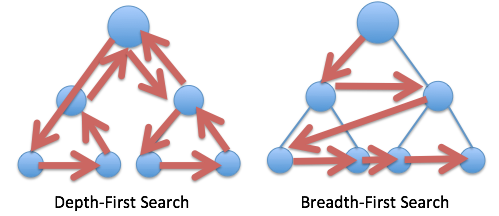
\includegraphics[width=0.5\textwidth]{img/depth-vs-breadth.png}
    \caption{Depth-First search vs Breadth-First search \cite{eppesHowComputerizedChess2019}}
\end{figure}

When that happens, that leaf node's position is evaluated and its value is returned
upwards to the parent node. The parent node looks at all of its children's values, 
and receives the maximum value when playing white, and the minimum value
when playing black. 

This repeats until the root node receives a value: the strength of the current position.

\subsubsection{The evaluation function}

The value estimation of leaf nodes is done by an evaluation function \cite{EvaluationFunction2022} written specifically
for the game. This function can differ from engine to engine, and is usually written with 
help from chess grandmasters. 



\subsubsection{Pseudocode}

The algorithm is recursive; it calls itself with different arguments, depending
on which player's turn it is. In chess, white wants to maximize the score, and 
black wants to minimize it. \cite{Minimax2022}

\begin{minted}{c}
function  minimax(node, depth, maximizingPlayer) is
    if depth = 0 or node is a terminal node then
        return the heuristic value of node
    if maximizingPlayer then
        value := - inf
        for each child of node do
            value := max(value, minimax(child, depth - 1, FALSE))
        return value
    else (* minimizing player *)
        value := + inf
        for each child of node do
            value := min(value, minimax(child, depth - 1, TRUE))
        return value
\end{minted}

Calling the function:

\begin{minted}{c}
// origin = node to start
// depth = depth limit
// maximizingPlayer = TRUE if white, FALSE if black
minimax(origin, depth, TRUE)
\end{minted}

\subsubsection{Alpha-beta pruning}

Because the necessary amount of nodes to get a good estimation of the strength of a position
is so high, the algorithm needs to be optimized. 
Alpha-beta pruning \cite{AlphaBetaPruning2022} aims to reduce the amount of nodes that need to be explored by minimax.
It does this by cutting off branches in the search tree that lead to worse outcomes.

Say you're playing the white pieces. You want to minimize your maximum loss, which means 
you want to make sure that black's score is as low as possible. 
Minimax always assumes that the opponent will play the best possible move. If one of white's possible moves
leads to a position where black gets a big advantage, it will eliminate that branch of the search tree.
As a result, the amount of nodes to explore is greatly reduced, while retaining a good estimation 
of the strength of the position.

\subsection{Monte Carlo Tree Search}

The biggest problem with minimax algorithms that use a depth limit is the dependency on the evaluation function.
If the evaluation function makes incorrect or suboptimal estimations, the algorithm will suggest bad moves. 
Developers of contemporary chess engines like StockFish continuously try to improve this function. 
Since 2020, StockFish has been using a sparse and shallow neural network as its evaluation function. 
This neural network is still trained using supervised learning, not (deep) reinforcement learning.

Using alpha-beta pruning can also bring about some problems. Say the player can sacrifice a piece
to get a huge advantage later in the game. The algorithm might cut off the branch and never explore that winning line, 
because it considers the sacrifice a losing position \cite{MinimaxMonteCarlo}. 

Monte Carlo Tree Search (MCTS) \cite{MonteCarloTree2022} is a search algorithm that can be used to mitigate these problems.
MCTS approximates the value of a position by creating a search tree using random exploration of the most promising moves.

\subsubsection{The algorithm}

To create this search tree for a certain position, MCTS will run the following algorithm hundreds of times. 
Each of these runs is called an MCTS \textbf{simulation}. One simulation consists of four steps:

\begin{enumerate}
    \item \textbf{Selection}:
    \begin{itemize}
        \item Starting from the root node, select a child node based on a formula of your choice.
        \item Most implementations of MCTS use some variant of Upper Confidence Bound (UCB) \cite{MLMonteCarlo2019}
        \item Keep selecting nodes until a node has been reached that has not been visited (=expanded) before. We call this a leaf node.
        \item If the root node is a leaf node, we immediately proceed to the next step.
    \end{itemize}
    \item \textbf{Expansion}:
    \begin{itemize}
        \item If the selected leaf node is a terminal node (the game ends), proceed to the backpropagation step.
        \item If it doesn't, create a child node for every possible action that can be taken from the selected node.
    \end{itemize}
    \item \textbf{Simulation}:
    \begin{itemize}
        \item Choose a random child node that was expanded in the previous step.
        \item By only choosing random moves, simulate the rest of the game from that child node's position.
    \end{itemize}
    \item \textbf{Backpropagation}:
    \begin{itemize}
        \item Return the simulation's result up the tree.
        \item Every node tracks the number of times it has been visited, and the number of times it has lead to a win.
    \end{itemize}
\end{enumerate}


\begin{figure}[H]
    \centering
    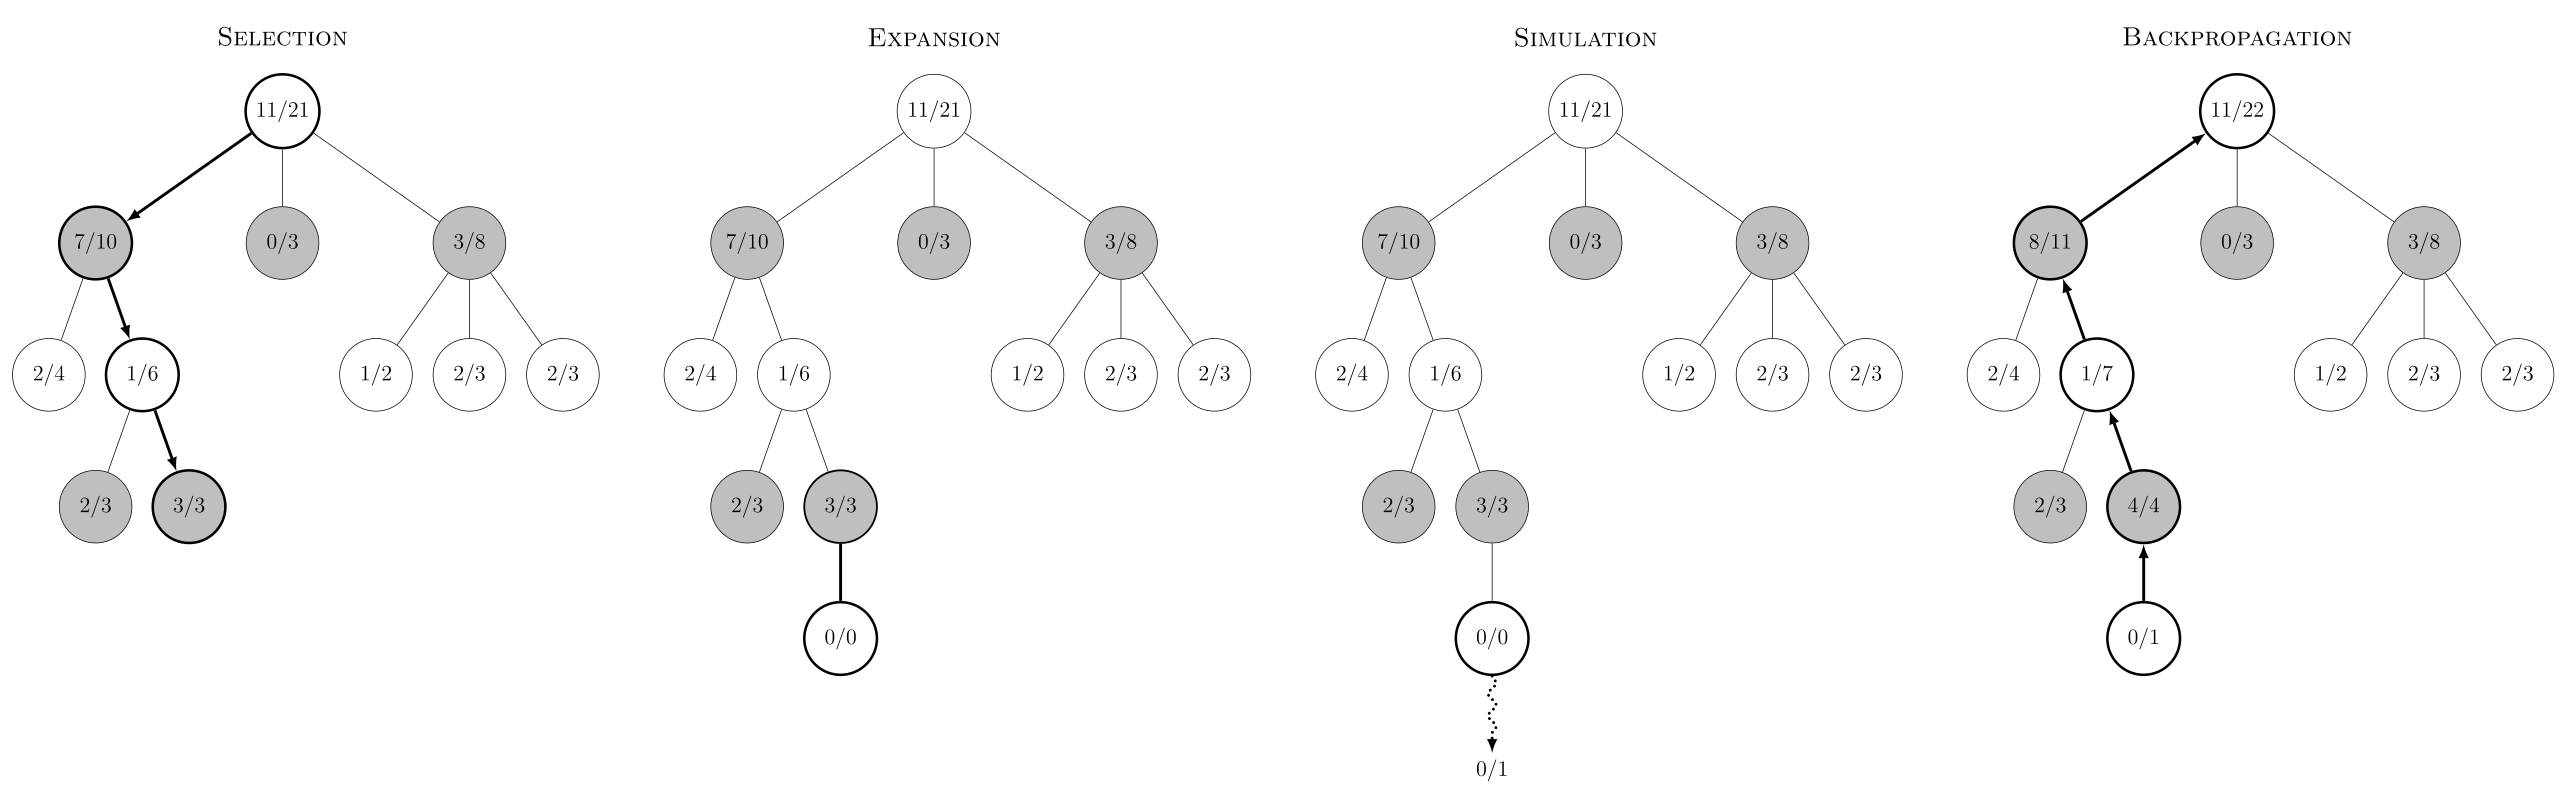
\includegraphics[width=0.98\textwidth]{img/MCTS-steps.png}
    \caption{The 4 steps of the MCTS algorithm \cite{MonteCarloTree2022}}
\end{figure}

For chess, this algorithm is very inefficient, because of its necessity to simulate 
an entire game of chess in the third step of every simulation. 
Just to calculate the value of one position would need hundreds of these simulations to get a good estimation.
This is why the selection formula needs to be chosen carefully; it's important to select nodes in a way that
balances exploration and exploitation.

\subsection{Go}

Go is a Chinese two-player strategy board game that uses white and black stones as playing pieces \cite{GoGame2022}.
It is played on a rectangular grid of (usually) 19 by 19 lines. The rules are relatively simple, but due to 
its extremely complex possibilities, Go has been a very popular playground for AI research similarly to chess.
Go's much larger branching factor compared to chess makes it very difficult to evaluate a position using 
traditional methods like minimax with alpha-beta pruning.

\begin{figure}[H]
    \centering
    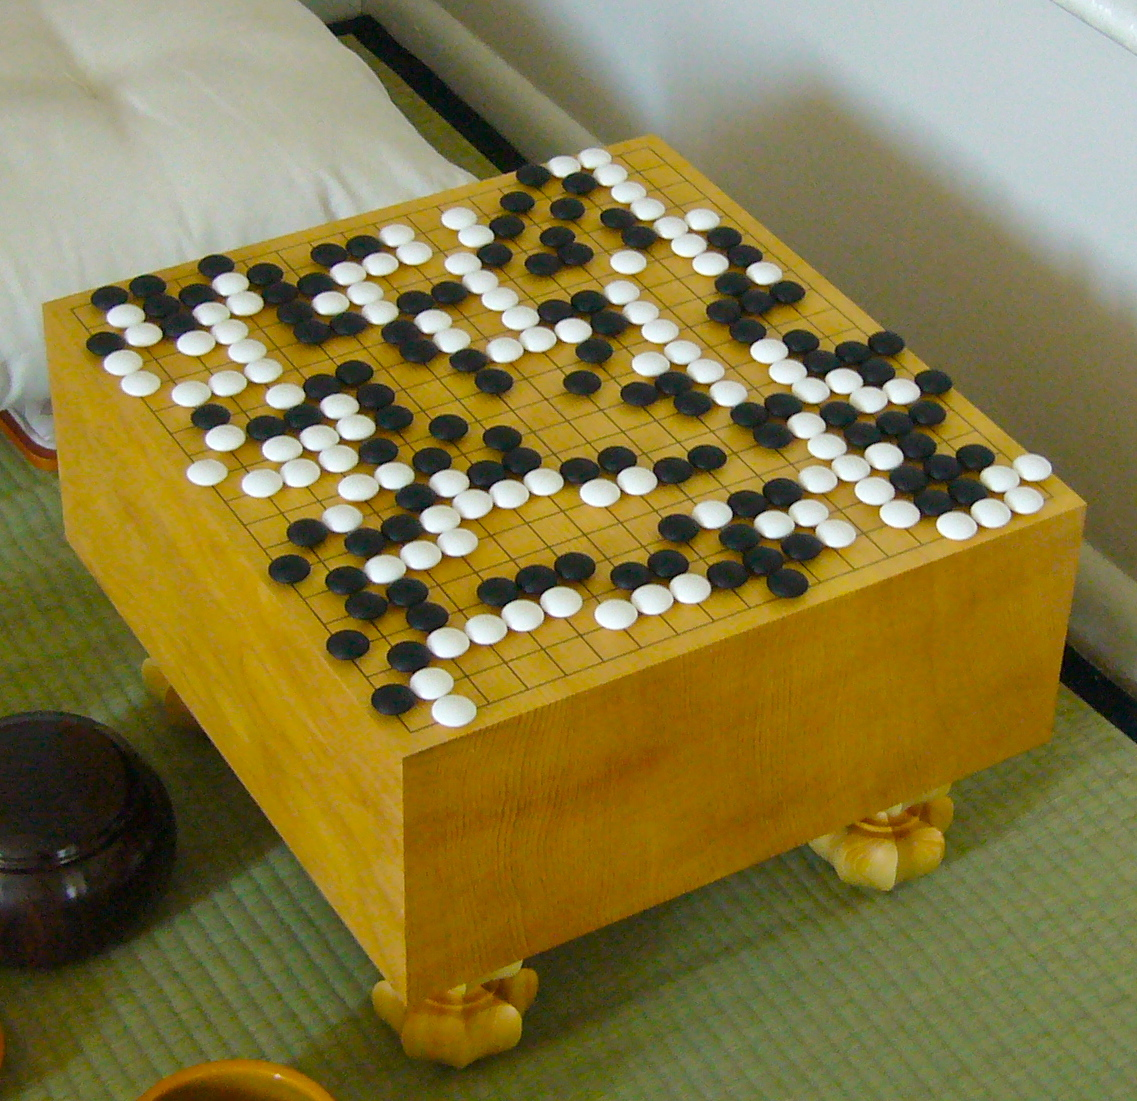
\includegraphics[width=0.5\textwidth]{img/go.jpg}
    \caption{Go board \cite{GoGame2022}}
\end{figure}

\subsubsection{AlphaGo}

In 2014, DeepMind Technologies \cite{DeepMind2022}, a subsidiary of Google, 
started developing a new algorithm called AlphaGo to play Go \cite{AlphaGo2022a}. 
Previously, the strongest Go engines were still only good enough to win against amateur Go players \cite{AlphaGo}.
The algorithm used a combination of the MCTS algorithm and a deep neural network to evaluate positions. 

AlphaGo was built \cite{AlphaGo} \cite{MasteringGameGo}  by first training a neural network with supervised learning by using data from human games.
The weights of that network were then copied to a new reinforcement learning network. That network was used to 
create a training set through self-play. By playing against itself and recording the board state, the 
moves the network considered, and the eventual winner of the game, a training set was created.
That training set was then used to train the reinforcement learning network. A separate network (the value network) 
was used to estimate the value of a position. 

\subsubsection{AlphaGo Zero}

Because AlphaGo still used some amateur games to learn from, the next step was creating a version of AlphaGo
that learns completely from scratch. That's why DeepMind developed AlphaGo Zero \cite{AlphaGoZero2022}.
AlphaGo Zero uses a different kind of network than AlphaGo. Instead of using two separate networks, 
it will combine the two outputs into a policy head and a value head. It's also using different layers:
residual layers instead of convolutional layers \cite{MasteringGameZero}. 

\subsection{AlphaZero}

AlphaZero is a generalized version of AlphaGo Zero, created to master the games of chess, shogi (``Japanese chess''), and Go \cite{AlphaZero2022} \cite{silverMasteringChessShogi2017c}. 
For chess, AlphaZero was evaluated against StockFish version 8 by playing 1000 games with 3 hours per player, plus 
15 seconds per move. It won 155 times, lost 6 times and the remaining games were drawn. 
AlphaZero uses a single neural network with two outputs, just like AlphaGo Zero. 


\subsubsection{Neural network input}

The input to the network represents the state of the game. 
It has the following shape: $N \cdot N \cdot (M \cdot T + L)$:

\begin{itemize}
    \item $N$ is the board size
    \begin{itemize}
        \item $N = 8$ in chess.
    \end{itemize}
    \item $M$ is the number of different pieces on the board, 
    \begin{itemize}
        \item Two players with six types of pieces each
        \item Every piece is represented by its own 8x8 board of boolean values
        \item For every square: $1$ if the piece is on that square, $0$ if it isn't
        \item $M = 12$ in chess
    \end{itemize}
    \item $T$ is the amount of previous moves that are used as input, including the current move. 
    \begin{itemize}
        \item AlphaZero used $T = 8$ for both chess, shogi, and Go.
        \item This gives the network a certain history to learn from
    \end{itemize}
    \item $L$ represents a set of rules specific to the game
    \begin{itemize}
        \item $L = 7$ in chess
        \item $1$ plane to indicate whose turn it is
        \item $1$ for the total amount of moves played so far
        \item $4$ for castling legality (white and black can both castle kingside or queenside under certain conditions)
        \item $1$ to represent a repetition count (in chess, 3 repetitions results in a draw)
    \end{itemize}
    \item $\Rightarrow 8 \cdot 8 \cdot (12 \cdot 8 + 7)$. 
\end{itemize}

This means that the input to the neural network is 119 8x8 boards of boolean values.

\subsubsection{Neural network layers}

DeepMind tested multiple neural network architectures for AlphaGo Zero \cite{NeuralNetworksChessprogramming}. 
The following parts were used in these networks:

\begin{itemize}
    \item Convolutional block
    \begin{itemize}
        \item A convolution layer
        \item Batch normalization layer
        \item ReLu activation function
    \end{itemize}
    \item Residual block
    \begin{itemize}
        \item This consists of two convolutional blocks, and a skip-connection
        \item The skip-connection will combine the input of the block to the output of the first two convolutional blocks
    \end{itemize}
\end{itemize}

These networks were tested by DeepMind during development of AlphaGo Zero \cite{MasteringGameZero}:

\begin{enumerate}
    \item \textbf{`dual-res':} a single tower of 20 residual blocks with combined policy and value heads. This is the architecture used in AlphaGo Zero.
    \item \textbf{`sep-res':} two towers of 20 residual blocks each: one with the policy head and one with the value head.
    \item \textbf{`dual-conv':} a single tower of 12 convolutional blocks with combined policy and value heads.
    \item \textbf{`sep-conv':} two towers of 12 convolutional blocks each: one with the policy head and one with the value head. This is the network used in AlphaGo.
\end{enumerate}

AlphaZero uses the same network architecture as AlphaGo Zero: dual-res.

\subsubsection{Neural network output}

The neural network has two outputs:

\begin{itemize}
    \item A policy head, which represents a probability distribution over the possible actions.
    \item A value head, which represents the value of the current position.
\end{itemize}

While the value head simply outputs a single float value between -1 and 1, the policy head is quite a bit more complicated.
It outputs a vector of probabilities, one for each possible action in the chosen game. 
For chess, 73 different types of actions are possible:

\begin{itemize}
    \item 56 possible types of ``queen-like'' moves: 8 directions to move the piece a distance between 1 and 7 squares.
    \item 8 possible knight moves
    \item 9 special ``underpromotion'' moves:
    \begin{itemize}
        \item If a pawn is promoted to a queen, it is counted as a queen-like move (see above)
        \item If a pawn is promoted to a rook, bishop, or knight, it is seen as an underpromotion (3 pieces)
        \item 3 ways to promote: pushing the pawn up to the final rank, or diagonally taking a piece and landing on the final rank
        \item $\Rightarrow 3 \cdot 3 = 9$
    \end{itemize}
\end{itemize}

These 73 actions are each represented by a plane of 8x8 float values. Say the first plane is a queen-like move
to move a piece one square northwest, the second plane could the same type of move, but a distance of two squares, and so on.
The squares on these planes represent the square from which to pick up a piece. 

% TODO: example

The result is a $73 \cdot 8 \cdot 8$ vector of probabilities, so $4672$ float values.  

\subsection{Training the network}

To train this type of network, it's necessary to create a dataset. 
This is done by letting the engine play against itself for a high amount of matches. 
Every move, data is collected and stored in a training set.
For complex games like chess, shogi and Go, this training set needs to be huge
because of the extremely large amount of possible situations.



\subsubsection{Tensor Processing Units (TPU)}

Because of the requirement to play a high amount of matches against itself, it was necessary to calculate
MCTS simulations in parallel on as fast as possible hardware. 
To help with these calculations, DeepMind used Google's newly created Tensor Processing Units (TPU) \cite{TensorProcessingUnit2022}.
A TPU is an application-specific integrated circuit (ASIC \cite{ApplicationspecificIntegratedCircuit2022}) that is specifically built for machine learning with
neural networks. Since 2018, these TPUs have been made publicly available to rent through Google's Cloud Platform. Smaller TPUs 
can be purchased from Google. 

\subsection{Leela Chess Zero}

Leela Chess Zero (lc0) is a free, open-source project that attempts to replicate the results of AlphaZero \cite{LeelaChessZero2022}. 
Lc0 was adapted from Leela Zero \cite{LeelaZero2021}, a Go computer that attempted to replicate the results AlphaGo Zero \cite{AlphaGoZero2022}. 

It is written in C++ \cite{Lc02022}, and it has managed to play at a level that is comparable to the current best version of StockFish.
Because lc0 is a community driven project, volunteers can help create training games through self-play using their own computers.
This made it possible to feed millions of chess games into the network. 

%%%%% Technical research %%%%%
\newpage
\section{Technical research}

% Volgende zaken worden verwacht:
% Beschrijving van de ontwikkelde software
% Opbouw applicatie: structuur/opbouw van het resultaat
% Achterliggende technologieën
% Overwonnen moeilijkheden/problemen
% …

\subsection{Introduction}

Creating the chess engine required programming the following parts:

\begin{itemize}
    \item The MCTS algorithm
    \item A tree data structure with nodes and edges
    \item The neural network
    \item The training pipeline
    \item The evaluation pipeline
    \item A way to store every move to a dataset
    \item A class to make the engine play against itself
    \item A GUI to play against the network
    \item Docker containers for easily scaling and distributing the program
\end{itemize}

All code was written in Python. The neural network was made using the TensorFlow Keras library.
Chess rules and helper functions were implemented using the open-source library python-chess \cite{PythonchessChessLibrarya}.

\subsection{Class structure}

\begin{figure}[H]
    \centering
    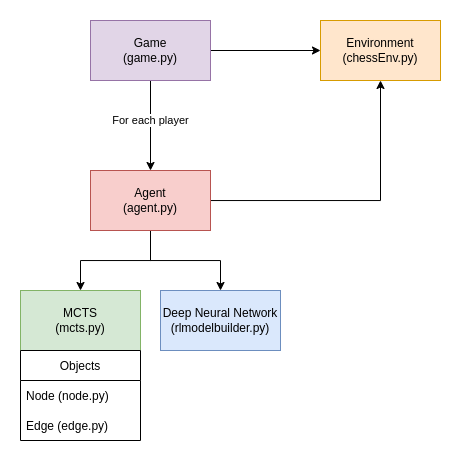
\includegraphics[width=0.6\textwidth]{img/class-structure.png}
    \caption{Basic class structure for the code responsible for playing a game}
\end{figure}

\subsubsection{Making one move}

\begin{figure}[H]
    \centering
    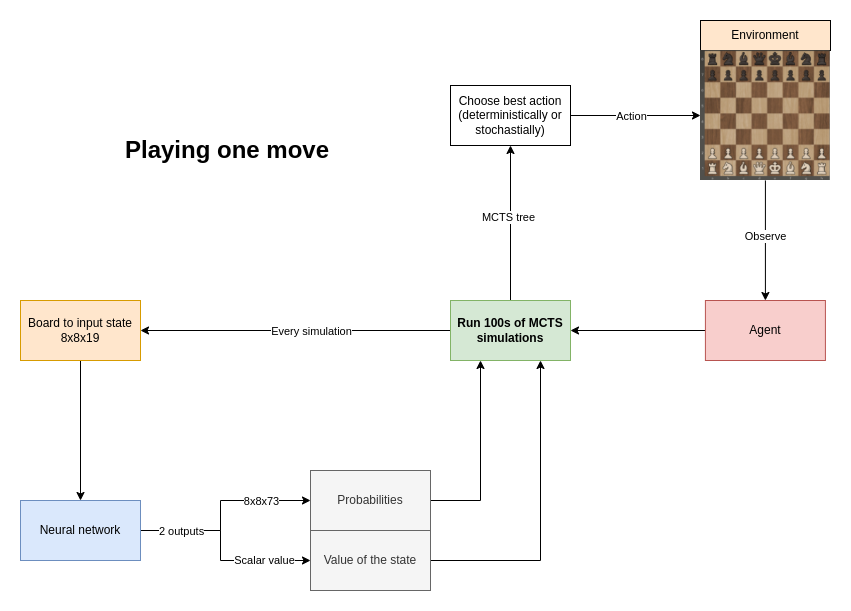
\includegraphics[width=0.95\textwidth]{img/ChessRL-schematic.png}
    \caption{Pipeline to make one move}
\end{figure}

To make a move, an Agent (white or black) observes the environment: the chessboard.
The agent calls upon the MCTS class to create a tree with as root the current state of the chessboard.
The MCTS class will run the MCTS algorithm hundreds of times. This amount is configurable in the config file. 
Higher amounts result in a more accurate estimation of the position's value, but also in longer 
computation times.

Every MCTS simulation, the neural network will be called to evaluate a position. The two outputs, 
the policy and the value, will be used to update the tree. 

\begin{figure}[H]
    \centering
    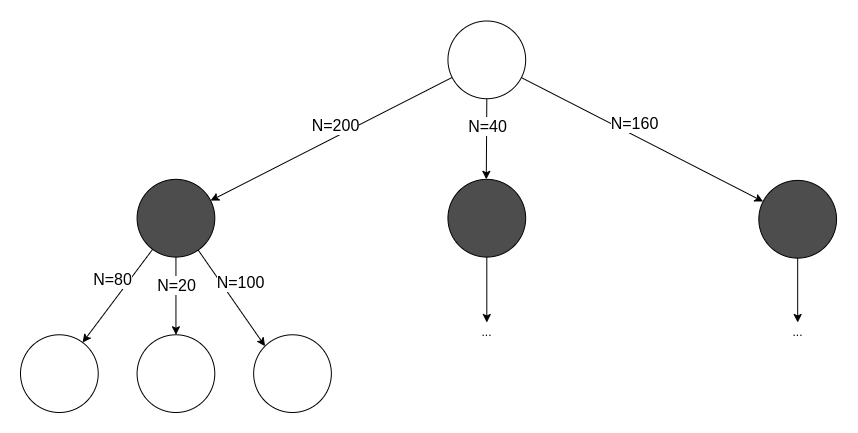
\includegraphics[width=0.65\textwidth]{img/MCTS-choose-move.png}
    \caption{Example tree after 400 simulations. N = amount of times the selection step selects that edge}
\end{figure}

After the simulations are done, the agent will pick the best move from the tree. 
It can do this in two ways:

\begin{itemize}
    \item Deterministically: choosing the most visited move 
    \item Stochastically: creating a uniform distribution of the visit counts and picking a move from that distribution
\end{itemize}

Stochastic selection is better when creating a training set, as it will result in a more diverse dataset.
Deterministic selection is better when evaluating with a previous network, or playing against the network competitively. 
In that case, picking the most visited move is the best choice.


\subsection{The neural network}

Initially, a prototype of the neural network was created with randomly initialized weights.
The Python class to create the model was immediately made with customizability in mind: 
the input and output shapes can be given as arguments, and the sizes of the convolution filters 
can be changed using a configuration file.

\subsection{A tree structure with nodes and edges}

As mentioned before, the MCTS algorithm creates a tree structure to represent 
the possible future states after the current position.

Node and Edge classes were written. The Node class represents a position in the game, and
holds the following data:

\begin{itemize}
    \item The position: a string representation of the board using the Forsyth-Edwards Notation (FEN) \cite{ForsythEdwardsNotation2022}
    \item The current player to move (boolean)
    \item A list of edges connected to this node
    \item The visit count of this node, initialized to 0
    \item The value for this node, initialized to 0
\end{itemize}

The Edge class represents a move. It holds the following data:

\begin{itemize}
    \item The input node (the position from which the move was made)
    \item The output node (the resulting position after taking the move)
    \item The move itself: an object of the Move class from the python-chess library, which holds:
    \begin{itemize}
        \item The source square and the target square of the move
        \item If the move was a promotion: the piece it was promoted to
    \end{itemize}
    \item The prior probability of this move
    \item The visit count of this edge, initialized to 0
    \item The value for this action, initialized to 0
\end{itemize}

The tree can also be plotted using the Graphviz library \cite{Graphviz}. A recursive function was written to 
create the tree and output it to an SVG file. 

\subsection{The MCTS algorithm}


\begin{figure}[H]
    \centering
    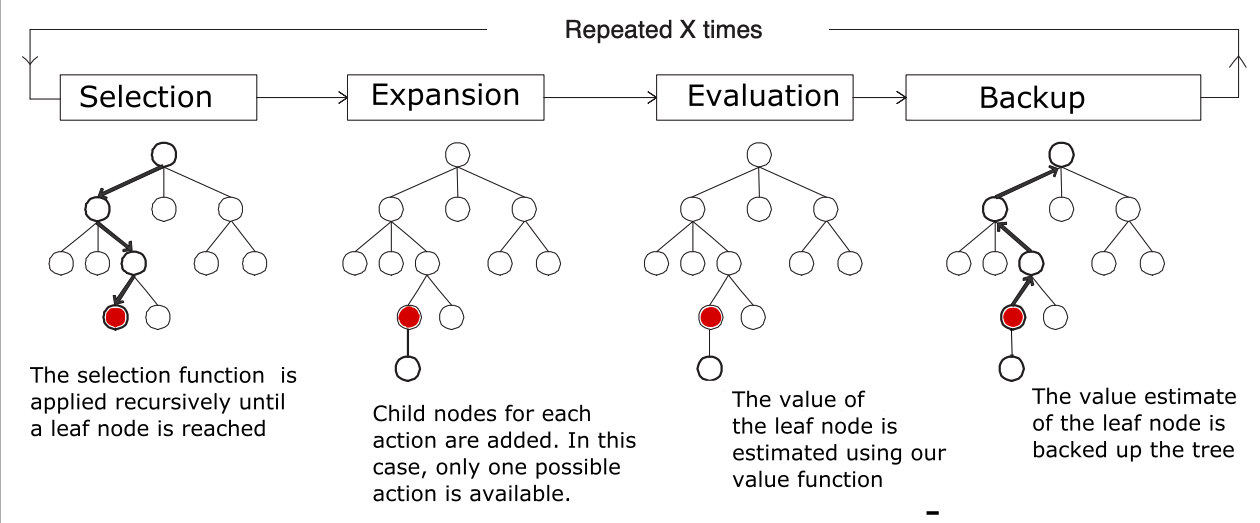
\includegraphics[width=0.9\textwidth]{img/mcts-alphazero.png}
    \caption{The four steps in AlphaZero's MCTS algorithm \cite{bodensteinAlphaZero2019}}
\end{figure}

A class was written to hold an MCTS tree. It holds the agent who created the tree and the
current position as the root node. 

\subsubsection{The selection step}

For the selection step, the following UCB formula was used to determine which edge to select:

\begin{center}
    \begin{equation}
        UCB = \Big(\log({\frac{(1 + N_{\text{parent}} + C_{\text{base}})}{C_{\text{base}}}}) + C_{\text{init}}\Big) \cdot P \cdot \frac{\sqrt{N_\text{parent}}}{(1 + N)}
    \end{equation}
\end{center}

\begin{itemize}
    \item $C_{\text{base}}$ and $C_{\text{init}}$ are constants that can be changed in the config file. The same values as AlphaZero were used.
    \item $N_{\text{parent}}$ is the visit count of the input node
    \item $N$ is the visit count of the edge
    \item $P$ is the prior probability of the edge
\end{itemize}

The selection step combines this UCB formula with the edges action-value and visit count:

\begin{center}
    \begin{equation}
        Q = \frac{W}{N+1}
    \end{equation}
\end{center}

\begin{center}
    \begin{equation}
        V = 
        \begin{cases}
            UCB + Q & \text{if white} \\
            UCB - Q & \text{if black}
        \end{cases}
    \end{equation}
\end{center}

The edge with the highest value ($V$) is selected. After selection, the 
visit count for the edge's output node is incremented by one. 
We call this output node the `leaf node'. 

\subsubsection{The expansion step}

The leaf node is expanded by creating a new edge for each possible (legal) move.
If there are no legal moves, the outcome (draw, win, loss) is checked and the leaf node
is passed to the next step in the algorithm.

If there are legal moves, the leaf node is given as an input to the neural network.
The neural network will return the policy and the value of the position.

As described in the research part of this thesis, the value is a float between -1 and 1, and the 
policy is a 73x8x8 tensor. This policy is mapped to a dictionary, where keys are moves and 
the values are the probabilities of each move. 

The neural network gets no information about the rules of chess, so it is necessary to filter
out the illegal moves. 

\begin{figure}[H]
    \centering
    
\includegraphics[width=0.95\textwidth]{img/output-planes/unfiltered.png}
    \caption{A subset of the 73 8x8 planes from the policy output. The brighter the pixel, the better the move. Grey padding was added to make a better visual presentation of the output planes.}
\end{figure}

\begin{figure}[H]
    \centering
    
\includegraphics[width=0.95\textwidth]{img/output-planes/filtered.png}
    \caption{The same subset, but with the illegal moves filtered out}
\end{figure}

The above two images were made using a trained model. The policy output of an untrained model with random weights 
looks like this:

\begin{figure}[H]
    \centering
    
\includegraphics[width=0.5\textwidth]{img/output-planes/random-model-unfiltered.png}
    \caption{Some output planes from an untrained model. Black padding was used to make it clearer.}
\end{figure}

This shows it is clear the trained model has some understanding of which moves are legal, 
without giving it any knowledge of the rules of chess. 

\subsubsection{The evaluation step}

The value received from the neural network is now assigned to the leaf node.

\subsubsection{The backpropagation step}

The value from the leaf node is now also added to every selected node in the path from the root to the leaf node.
Concretely, for every selected edge in the path, the following values are changed:

\begin{itemize}
    \item The edge's input node's visit count is incremented by 1
    \item The edge's visit count is incremented by 1
    \item The edge's value is incremented by the value of the leaf node
\end{itemize}


\subsection{Saving training data}


\begin{figure}[H]
    \centering
    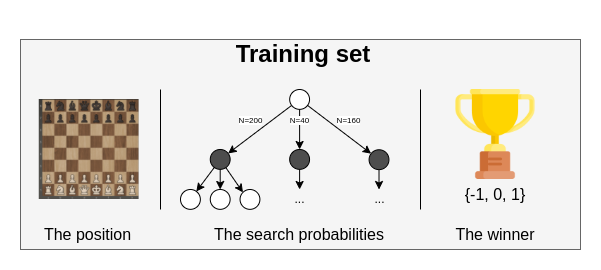
\includegraphics[width=0.7\textwidth]{img/trainingset.png}
    \caption{The training set consists of: the input state, the move probabilities, and the eventual winner}
\end{figure}

Every move is saved to memory in a simple Python list. Once the game is over, the winner is added to every move in memory.
The whole game is then saved to a binary file in NumPy's .npy format. 
When a new game starts, the memory is cleared.

\subsection{Training the neural network}

\begin{figure}[H]
    \centering
    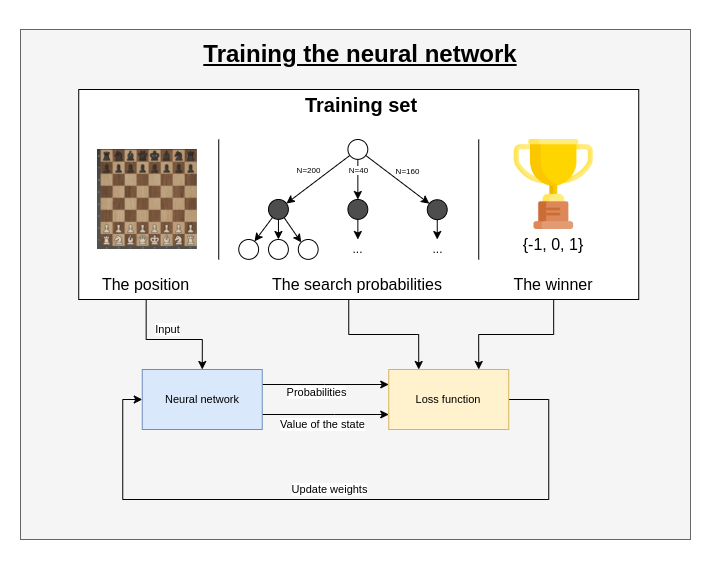
\includegraphics[width=0.9\textwidth]{img/training.png}
    \caption{The training pipeline}
\end{figure}

To train the neural network, every saved game's binary file is loaded 
into memory. The memory is shuffled to avoid the neural network accidentally learning
time dependent patterns. Random batches of the training set are then processed through the
neural network.

The position is used as the input to the neural network. The network's outputs are then 
compared to the move probabilities and the winner from the dataset:

\begin{itemize}
    \item The move probabilities are converted to a 73x8x8 tensor, which is compared with the output of the network
    \item The winner is compared with the value output of the network.
\end{itemize}

The training pipeline employs two separate loss functions. The policy head uses categorical cross-entropy
and the value head uses mean squared error.

\subsection{Multiprocessing}

\subsection{The final project}

% the files in the project

\subsection{Porting to C++}




%%%%% Reflection %%%%%
\newpage
\section{Reflection}

%%%%% Advice %%%%%
\newpage
\section{Advice}

%%%%% Conclusion %%%%%
\newpage
\section{Conclusion}

%%%%% Bibliography %%%%%
\newpage
\section{Bibliography}
\renewcommand{\bibname}{}
\printbibliography[heading=none]

%%%%% Appendix %%%%%
\newpage
\section{Appendix}





\end{document}